\thesis{\section{Sensitivity to Signal Shape Mismatch}}
\note{\section{Sensitivity to Signal Shape Mismatch}}
\label{sec:shape_mismatch}

The model-independent scan uses a single signal shape to represent all benchmark models, even though the true resonance width varies between them.
To quantify the resulting loss in sensitivity, three representative signal shapes spanning the range of widths present in the benchmark models -- narrow (VLL), medium (TP), and wide ($H_2 \to H_1 H_3$) -- are injected as real signal simulation events into the anomaly-selected background at four masses, 15, 35, 55 and 75\GeV, at a strength calibrated to give a discovery significance of approximately $5\sigma$ when fit with the matching template.
Each injected sample is then fit with all three templates in turn, isolating the loss in discovery significance due to a mismatch between the true signal shape and the template assumed in the fit.
For each of the twelve (injected shape, template) combinations at each mass, ten pseudo-datasets are generated (bootstrapped background plus Poisson-fluctuated signal) and fit, and the mean significance and its standard error are reported.

The results are shown in Fig.~\ref{fig:shape_mismatch_z}.
The matched-template significance is close to the calibration target ($4.5$--$5.8\sigma$) at all four masses.
Away from the diagonal, the loss in significance is small everywhere except for a narrow signal fit with the wide template at 15\GeV, where the significance drops from $4.58 \pm 0.33$ to $2.82 \pm 0.34$, a loss of about 39\%.
This is the region where the three widths differ most (by a factor of about three at 15\GeV, compared to about 1.3 at 75\GeV), and a template narrower than the truth costs comparatively little, while a template wider than the truth suppresses the peak significantly.
At 55 and 75\GeV, where the widths of the three benchmark classes converge, every mismatch combination costs less than 10\% of the matched significance.

\begin{figure}[h!]
    \centering
    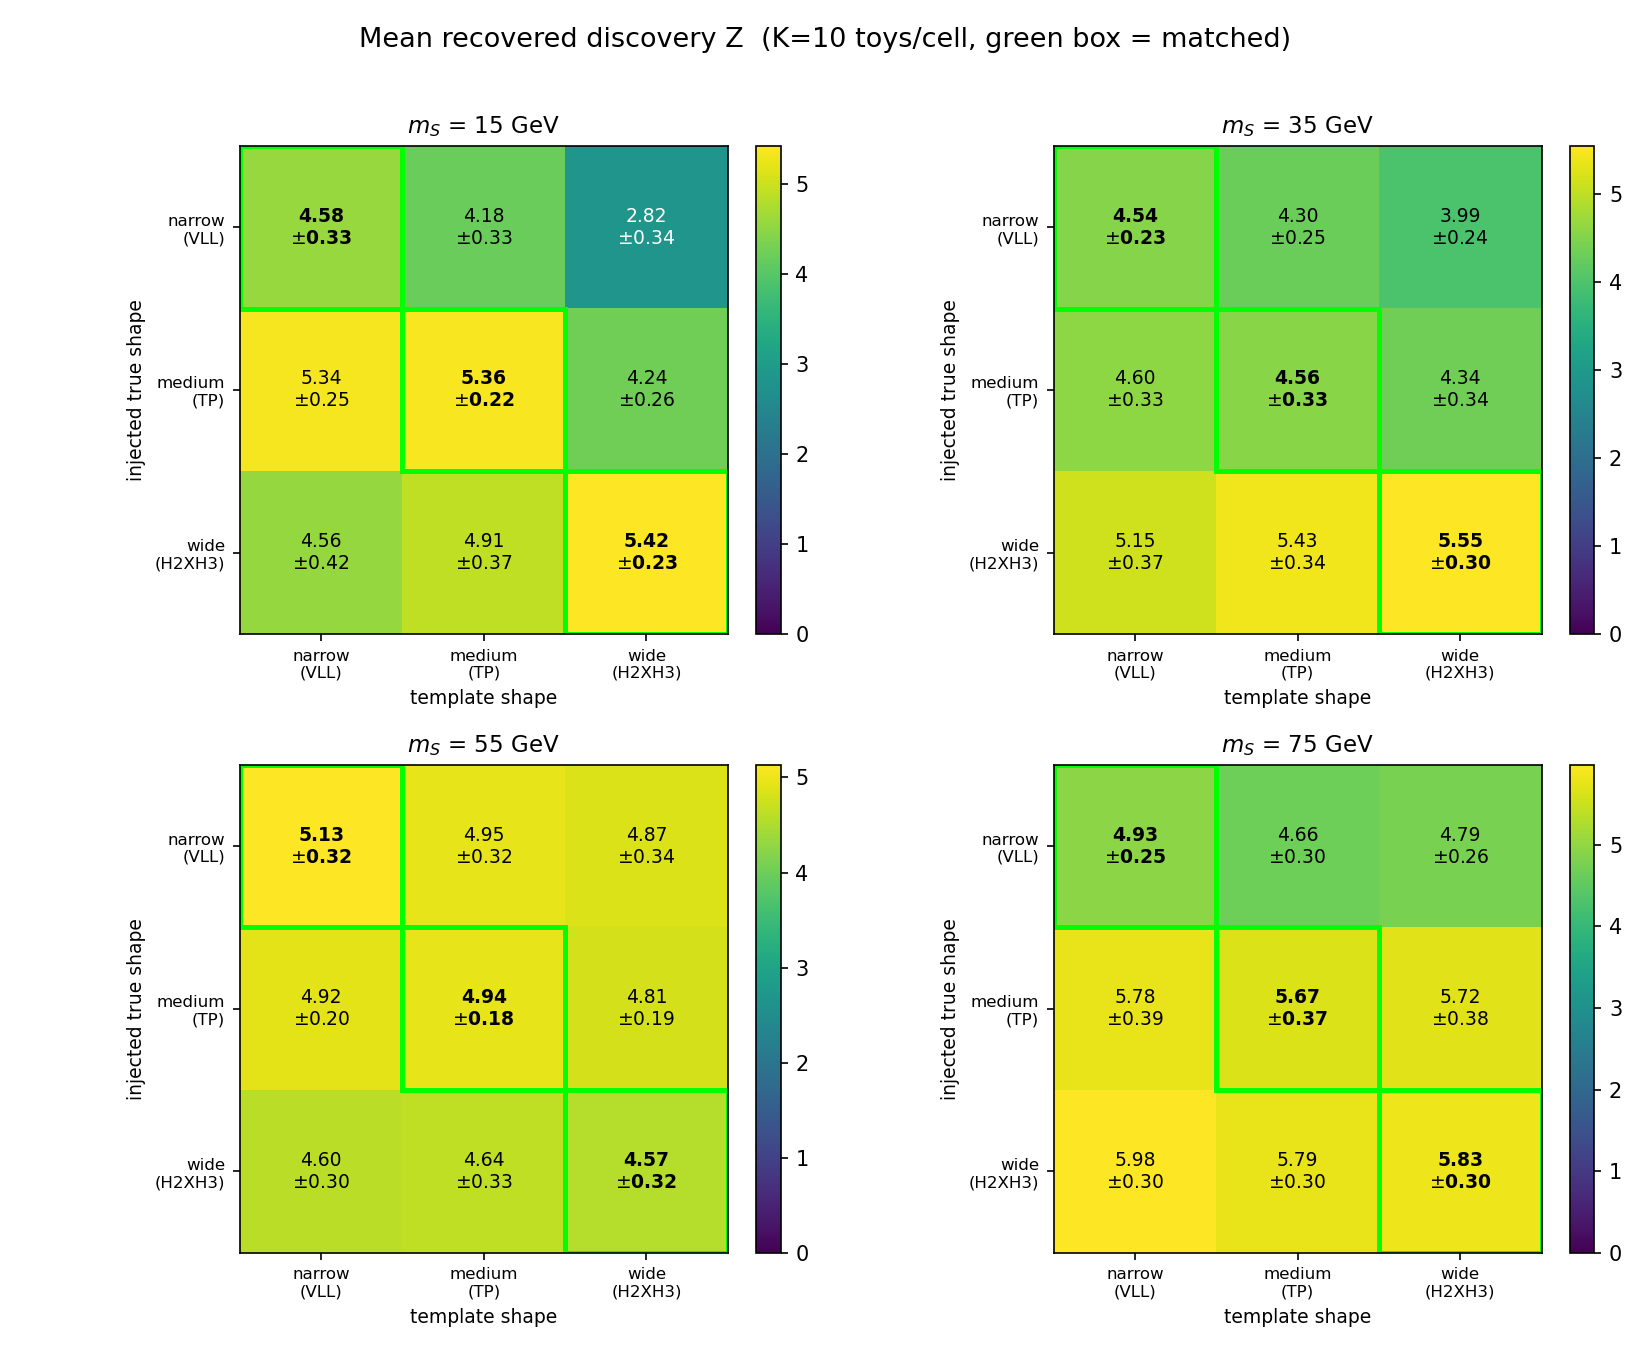
\includegraphics[width=0.95\linewidth]{Figures/Appendix_ShapeMismatch_figures/shape_mismatch_Z.png}
    \caption{Mean recovered discovery significance (with standard error on the mean, from ten pseudo-datasets per cell) as a function of the injected signal shape (rows) and the template used in the fit (columns), at four representative masses. The matched (correct-template) cell in each row is outlined in green.}
    \label{fig:shape_mismatch_z}
\end{figure}

Because the medium-width template minimizes the worst-case loss in discovery significance across the three benchmark shapes -- most importantly at low mass, where the shapes differ most -- the medium-width signal shape is adopted as the single template used in the model-independent scan.
